%% PKU-style slide template
%
%% pkuslideTemplate.tex
%
% Written by pppppass (lzh2016p@pku.edu.cn), this file belongs to
% public domain.
%
% Further information can be found in
%   pkuslide.manifest.md
% and
%   Readme.md
% and an introduction to the whole project is included as well.

% !TeX encoding = UTF-8 Unicode
% !TeX program = LuaLaTeX
% !TeX spellcheck = LaTeX

% Author : pppppass
% Description : PKU-style slide template

\documentclass[english]{pkuslide}

\usepackage[cmrgreekup]{def}
\addbibresource{TemplateBibliography.bib}

\newtheorem{Thm}{Thm}
\newtheorem{ColoredThm}{ColoredThm}

\definecolor{nonpkupurple}{HTML}{c71585}
\AtBeginEnvironment{ColoredThm}{%
\setbeamercolor{block title}{use=example text,fg=gray!10,bg=nonpkupurple!75!bg}%
}

\title[模型检验]{基于逆推算法和深度优先搜索的模型检验}
\subtitle{数据结构大作业}
\institute{北京大学数学科学学院}

\author{王逸轩、韩啸}
\date{\today}

\subject{模型检验}
\keywords{模型检验,迁移状态系统,线性时序逻辑,计算树逻辑}

	\begin{document}

	\begin{frame}
\titlepage
	\end{frame}

	\begin{frame}
\tableofcontents[subsectionstyle=show]
	\end{frame}

\section{问题分析}
\frame{\sectionpage}
\subsection{背景}
\begin{frame}{基本术语}
\begin{itemize}[<+->]
\item 迁移状态系统$TS$;
\item 逻辑公式$L$;
\item 公式类型$LTL$、$CTL$等;
\item 公式基本算符.
\end{itemize}
\end{frame}
\begin{frame}{问题的关联}
从给定的迁移状态系统出发,我们研究不同的逻辑公式,发现本质上就是针对对象的不同。
\begin{figure}
\centering
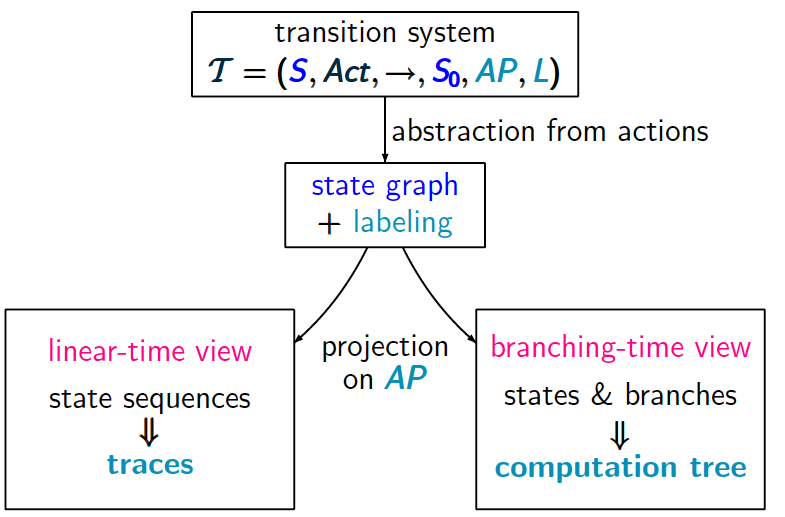
\includegraphics[height=0.5\textheight]{1.png}
\caption{PPT中刻画$CTL$与$LTL$模型检验的关联}
\end{figure}
\end{frame}
\begin{frame}{两个例子}
\centering
\begin{alertblock}{我们具体考察$CTL$与$LTL$模型检验的两个简单实例。}
\end{alertblock}
\end{frame}
\begin{quoteslide}
\includepdf[pagecommand=\quotefootnote{$CTL$模型检验}, pages=98, scale=0.8]{lec16.pdf}
\end{quoteslide}
\begin{quoteslide}
\includepdf[pagecommand=\quotefootnote{$LTL$模型检验}, pages=92, scale=0.8]{lec1213.pdf}
\end{quoteslide}
\subsection{解决方案}
\begin{frame}{待解决的问题}
\begin{enumerate}[<+->]
\item 刻画迁移状态系统$TS$;
\item 刻画逻辑公式$L$;
\item 建立对公式的一些运算法则(如取子式、递推等等);
\item 针对不同的公式类型,设计算法.
\end{enumerate}
\end{frame}
\begin{frame}{问题难点}
\begin{enumerate}
\item 如何刻画初始的输入信息;
\item $CTL$可以利用朴素的逆推方法解决,如何定位子串;
\item $LTL$中逆推算法可能无限循环,找到替代方案处理“无穷”的问题;
\item 通过逻辑筛选,简化枚举次数,降低时间复杂度.
\end{enumerate}
\end{frame}
\begin{frame}{处理问题的思想}
\begin{enumerate}
\item 用图结构储存迁移状态系统$TS$;
\item 用字符串存储逻辑公式$L$,并假设已指明逻辑类型并添加括号;
\item 对$CTL$公式,利用建立的运算法则,逆推判断;
\item 对$LTL$公式,利用公式的所有子串的满足情况构建新的图,深度优先搜索举例.
\end{enumerate}
\end{frame}

\section{算法设计}

\frame{\sectionpage}
\subsection{$CTL$算法设计}
	\frame{\subsectionpage}
\begin{frame}{逆推算法}{算法的指导思想}
\onslide<1->{本质上的思想是找到每个逻辑公式对应的满足该公式的节点集合。}

\onslide<1->{}

\onslide<1->{解决了最简单的公式对应的节点集合之后,就可以对于复杂的公式,利用逆推算法,脱去最外层的括号,找到相应的节点集合。}

\onslide<1->{}

\onslide<1>{最后通过原始逻辑公式$L$找到的相应节点集合,判断迁移状态系统$TS$的初始节点是否在该集合中即可。}
\end{frame}
\begin{frame}{逆推算法}{需要注意的问题}
尽管我们结合前面的分析,知道逆推算法能够有效的解决$CTL$模型检验问题,但我们还需要注意处理以下的细节。
\begin{enumerate}
\item 括号匹配:我们在逆推时需要定位最左侧括号对应的反括号,进而分割出完整的子式语句;
\item 最外层算符的讨论:我们在逆推时需要特别注意,最外侧为${\forall}$、${\exists}$这两个算符时,要连同下一个算符一起考虑。
\end{enumerate}
\end{frame}
\subsection{$LTL$算法设计}
	\frame{\subsectionpage}
\begin{quoteslide}
\includepdf[pagecommand=\quotefootnote{利用$NBA$解决$LTL$模型检验}, pages=33, scale=0.8]{lec1314_reduced.pdf}
\end{quoteslide}

\begin{frame}{克服逆推算法带来的“无穷”的问题}
如前所述,朴素的逆推算法难以解决$LTL$模型检验的问题,我们参阅\nocite{*}\href{https://moves.rwth-aachen.de/teaching/ss-16/ss16introduction-to-model-checking/}{\emph{Introduction to Model Checking}}这门课程的PPT资源,利用$NBA$找到了以下代替方案:

我们把逻辑公式$S$的所有子串给记录下来,然后这些子串形成一个集合,我们考察这个集合生成的子集族$Q$,子集族中每个元素代表着相应的子串得到了满足,而余下的子串没有得到满足。我们考察一个新的图$G_{1}$,节点集合是由原来的节点集合$V$与新得到的子集族$Q$形成的的笛卡尔积,我们设法把原来的迁移状态系统$TS$存在反例的问题转化为新图$G_{1}$存在一条满足某种性质的路径的问题,这样一来通过对$G_{1}$的深度搜索即可完成结论。
\end{frame}
\begin{frame}{理论支持}
首先我们需要说明原来的迁移状态系统$TS$存在反例,就等价于新图$G_{1}$中存在某种无穷长的路径。这在PPT的如下定理中得到佐证。
\begin{figure}
\centering
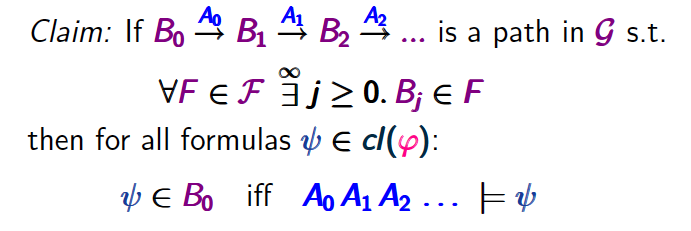
\includegraphics[height=0.4\textheight]{Figure_1.png}
\end{figure}
其次,我们说明给出的反例一定可以具有无穷循环的回路的形式。这个事实我们通过回路的拼接可以说明。
\end{frame}
\begin{frame}{核心算法的描述}
结合之前的理论支持,我们把寻找反例转化为找到在$G_{1}$中的一个无穷路径,其中有限步之后形成回路的无穷循环,这个回路满足所有出现的无穷算符。最后一步,我们通过深度优先搜索来实现。
\end{frame}
\begin{frame}{具体算法的设计}
我们简明扼要地给出算法的步骤:
\begin{enumerate}[<+->]
\item 简化输入的$LTL$公式,用$U$“直到”算符来表示$W$“弱直到”、$D$“最终满足”、$S$“一直满足”等算符
\item 找到那些出现$U$“直到”算符,即需要之后回路判断的子串
\item 先进行一步筛查来判断哪些图$G_{1}$中的点连有边,即原图$G$中哪些状态可以相互转化
\item 最后对于图$G_{1}$进行深度优先搜索,判断是否存在满足反例条件的回路
\end{enumerate}
\end{frame}
\section{模型展望}
\frame{\sectionpage}
\subsection{模型的评价}
\begin{frame}{模型的优点}
\begin{enumerate}
\item 处理$CTL$模型检验时,我们的算法在思想上和具体实现上都十分简单,程序的复杂度也很低,我们可以容易地处理大规模的模型检验运算。
\item 处理$LTL$模型检验时,我们的算法将反例化归到回路情况,能够较好地给出反例。
\item 我们将输入输出标准化,存储在文件里,判断具体的模型检验时就显得一目了然了。
\end{enumerate}
\end{frame}
\begin{frame}{模型的缺点}
\begin{enumerate}
\item 在$LTL$模型检验中,我们的程序在时间复杂度和空间复杂度上都显得太过于复杂,深度搜索引入了近乎难以容忍的运算量,于是$LTL$的算法只能解决比$CTL$模型检验规模小的多的问题。
\item 程序的交互性做的不够好,不能达到一个较好的可视化界面的设计。
\end{enumerate}
\end{frame}
\subsection{模型的推广}
\begin{frame}{$CTL$*模型检验}{定义}
\begin{figure}
\centering
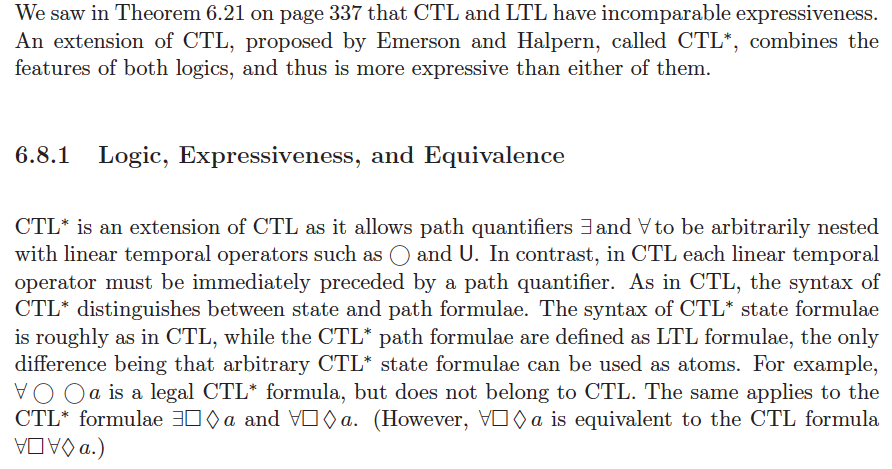
\includegraphics[height=0.5\textheight]{2.png}
\end{figure}
\end{frame}
\begin{frame}{$CTL$*模型检验}{算法}
$CTL$*模型检验,在本质上是$LTL$与$CTL$模型检验算法的整合,我们利用逆推算法来拆解$CTL$*逻辑公式,在必要的逆推步骤时利用$LTL$模型检验得到的结果。
\begin{figure}
\centering
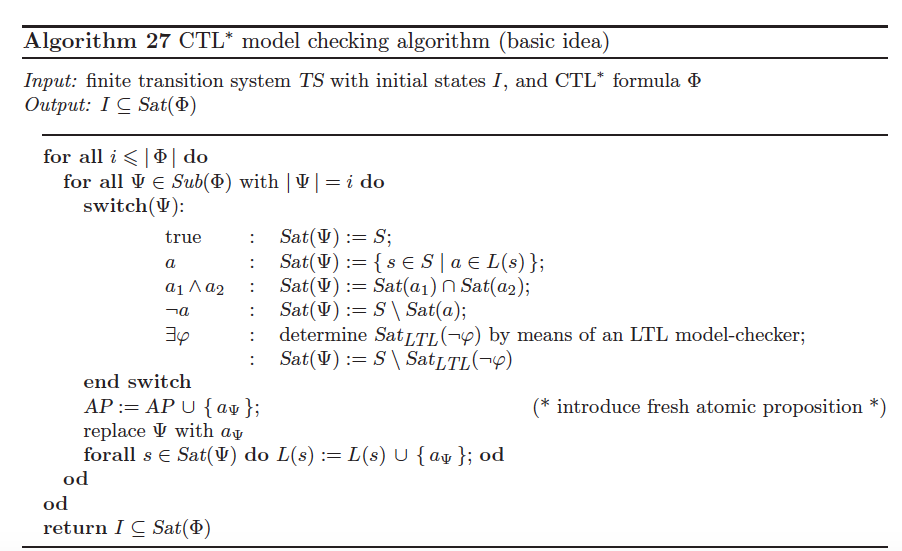
\includegraphics[height=0.5\textheight]{3.png}
\end{figure}
\end{frame}
\begin{frame}{$TCTL$模型检验}{探索}
本质上$TCTL$就是考虑到时间因素的$CTL$模型,逆推的过程中考虑时间元素即可。
\end{frame}
\begin{frame}{$PCTL$模型检验}{展望}
$PCTL$中状态出现的概率也可以朴素的使用逆推来完成计算,并比较输出检验成果。
\end{frame}
\section{参考书目}
\begin{frame}{参考书目}
\printbibliography
\end{frame}
\section{结束语}
\begin{frame}
\LARGE
\begin{beamercolorbox}[center, ht=3em]{titlelike}
\vspace{1em}
谢谢!
\end{beamercolorbox}
\end{frame}
\end{document}
